

\section{Atmospheric Neutrino Fit Results}
\label{sec:fitresults}

Following the approach outlined in the previous section, we fit all 288
parameters for the atmospheric flux, cross section, and detector systematics to
the atmospheric data by running a sequence of Markov chains.  An initial MCMC is
performed with approximately two million steps to build up the distributions of
the differential parameters.  We then draw from these distributions when running
an additional two million steps of DE-MCMC\@.  The final output of this fit is 
a sampling of the (correlated) fit parameters that best agree with data. The parameter
correlations are visualized in Figure~\ref{fig:fitcorr}.

\begin{figure}[h]
  \begin{center}
    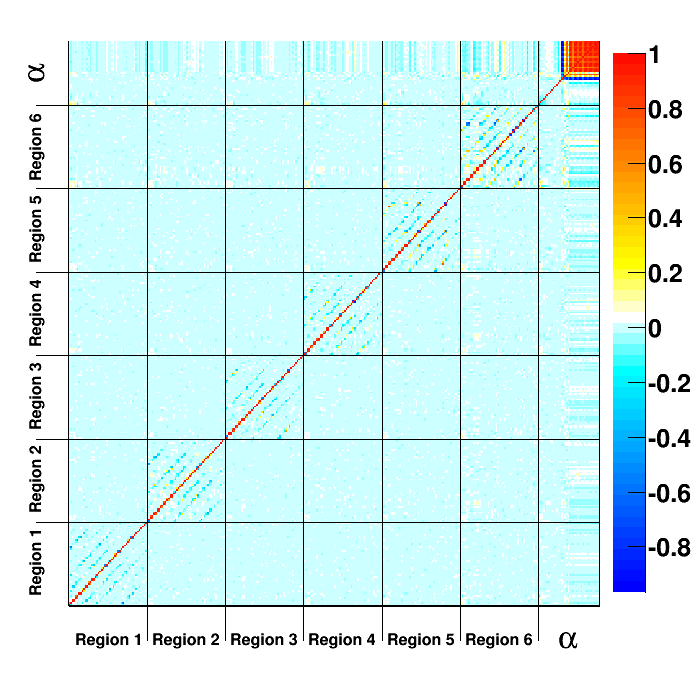
\includegraphics[width=0.7\textwidth]{hcorr_full_labeled}
  \end{center}
  \caption{Correlation matrix for all 288 parameters in the atmospheric fit.
  The labeled regions correspond to the SK detector regions defined in
  Section~\ref{subsec:DR}.  The region labeled $\alpha$ contains all of the
  flux, cross section, and normalization parameters.}
  \label{fig:fitcorr}
\end{figure}

To analyze the fit results, we
sample points from the DE-MCMC result and apply them to the simulated
atmospheric data\@.  In each histogram bin, we can calculate the mean and
statistical variance of the fit result, which is used to calculate the
statistical error.  Ideally, the observed data should be consistent with the
post-fit MCMC mean within the statistical error.  We find the average deviation
from the post-fit mean in each bin to be $1.11\sigma$, where $\sigma$ denotes
the statistical error of that bin.  The detailed fit results for each of the
histograms compared between data and MC can be seen in
Figures~\ref{fig:fitresults_samp0_att0}-~\ref{fig:fitresults_samp2_att3}.

%% ATTRIBUTE 0 %%%%%%%%%%%%%%%%%%%%%%%%%%%%%%%%%%%%%%%%%%%%%%%%%%%%%%%%%%%%%%%%%%%
\begin{figure}[h]
  \begin{center}
    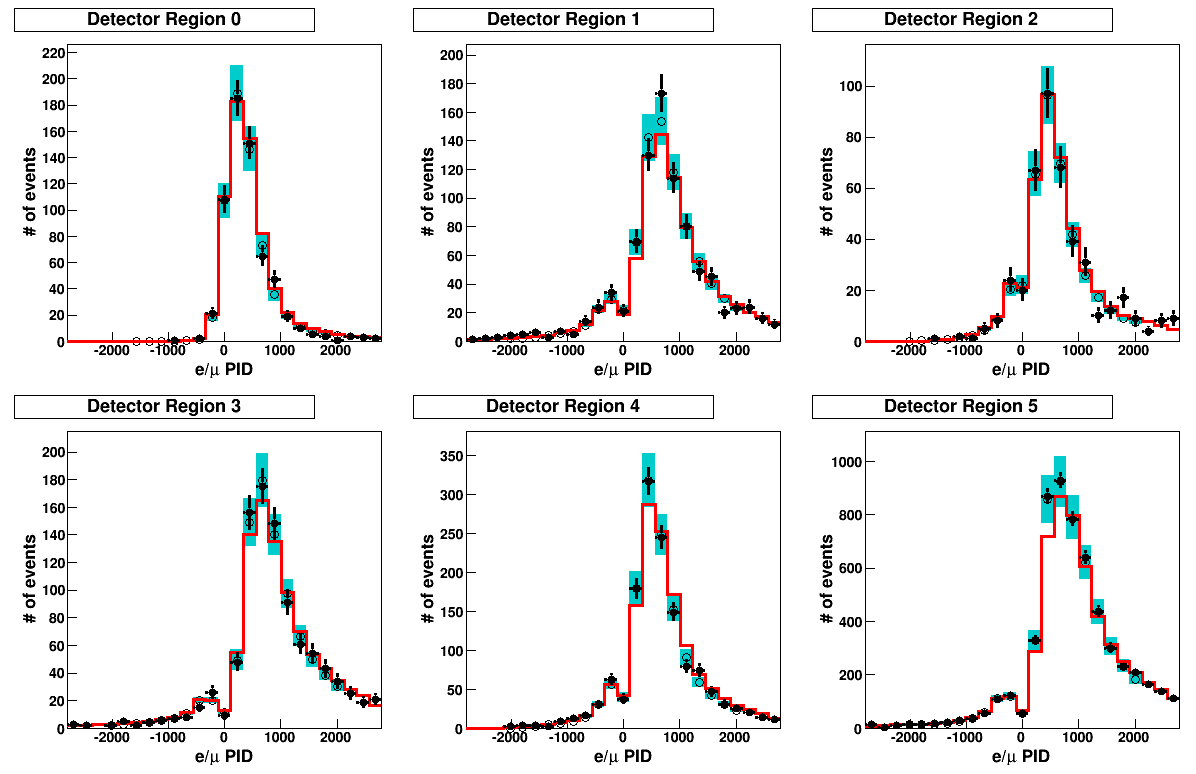
\includegraphics[width=0.9\textwidth]{demcmc_fitresult_samp0_attribute0} 
  \end{center}
  \caption{Fit results for the $l=0$ control sample (no decay electrons) for
  the fiTQun $e/\mu$ PID variable in each of the detector regions.  Positive
  values denote more $e$-like events, negative values denote more $\mu$-like
  events.  Red histogram shows nominal MC prediction.  Black points represent
  observed data.  Teal histogram shows post-fit distribution, where the mean is
  the average of the DE-MCMC throws and the error bar is the square root of the
  variance.}
  \label{fig:fitresults_samp0_att0}
\end{figure}


\begin{figure}[h]
  \begin{center}
    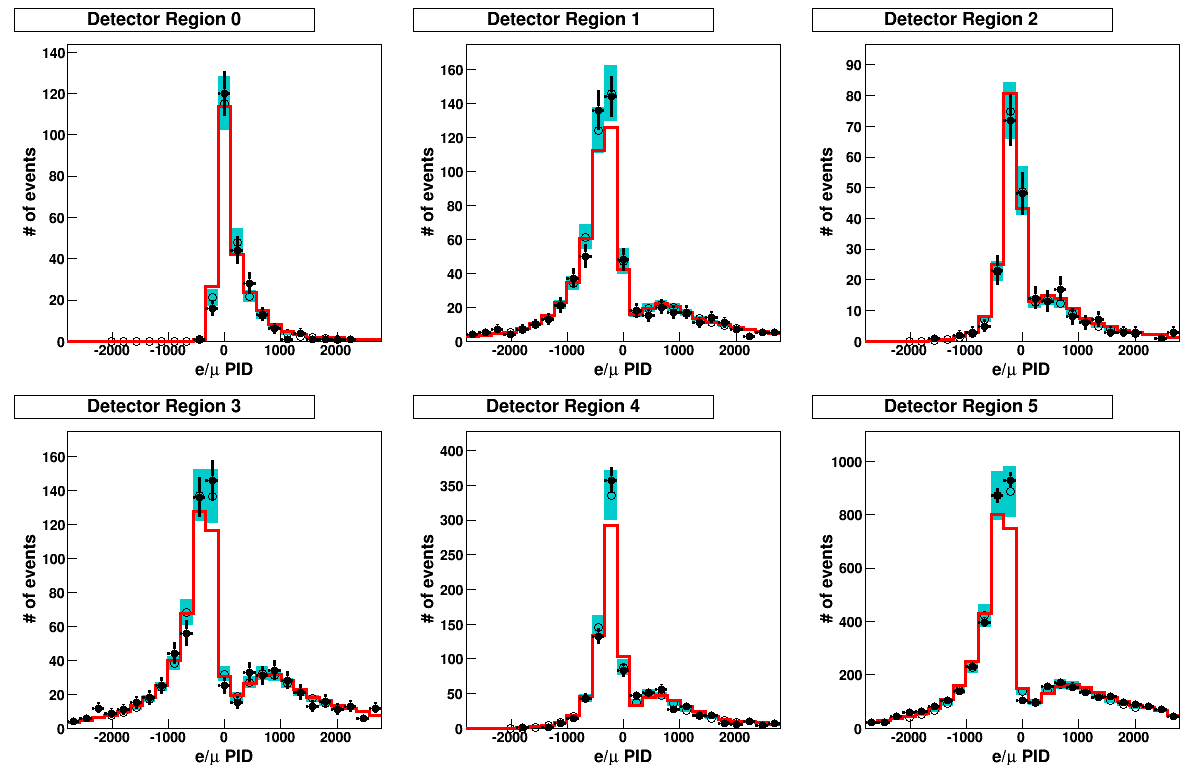
\includegraphics[width=0.9\textwidth]{demcmc_fitresult_samp1_attribute0} 
  \end{center}
  \caption{Fit results for the $l=1$ control sample (one decay electron) for
  the fiTQun $e/\mu$ PID variable in each of the detector regions.  Positive
  values denote more $e$-like events, negative values denote more $\mu$-like
  events.  Red histogram shows nominal MC prediction.  Black points represent
  observed data.  Teal histogram shows post-fit distribution, where the mean is
  the average of the DE-MCMC throws and the error bar is the square root of the
  variance.}
  \label{fig:fitresults_samp1_att0}
\end{figure}


\begin{figure}[h]
  \begin{center}
    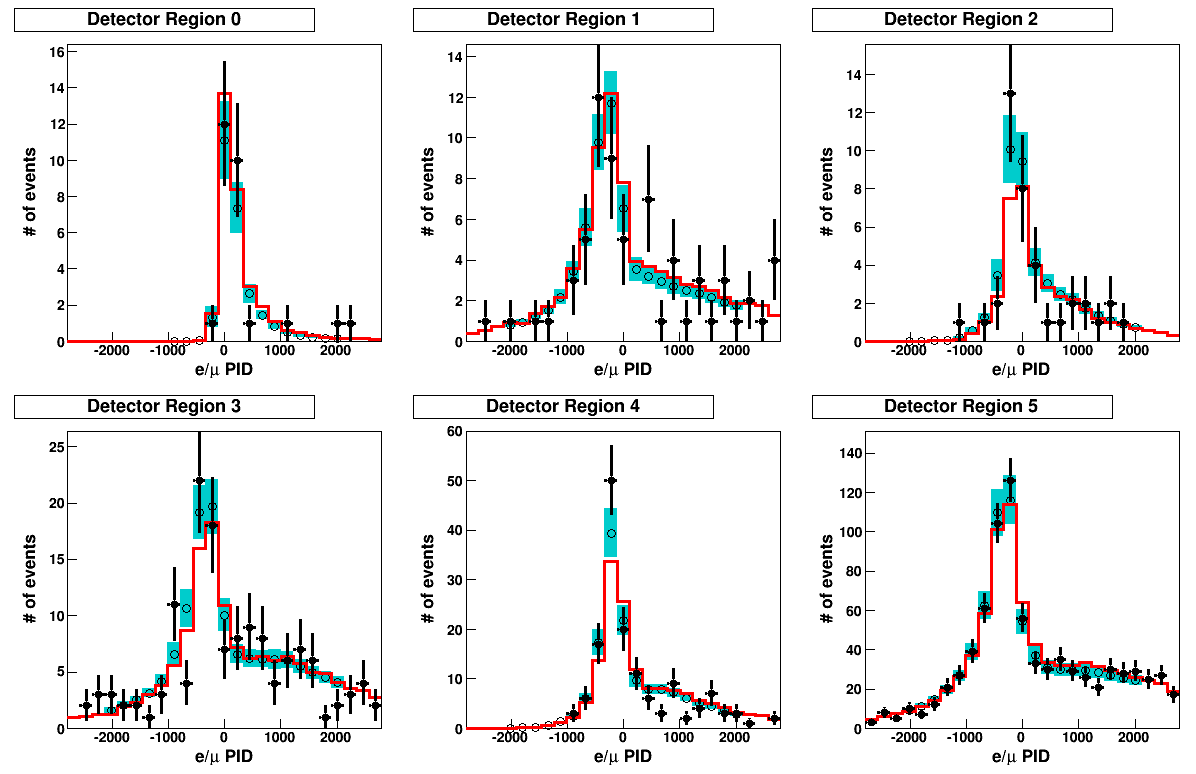
\includegraphics[width=0.9\textwidth]{demcmc_fitresult_samp2_attribute0} 
  \end{center}
  \caption{Fit results for the $l=2$ control sample (more than one decay
  electron) for the fiTQun $e/\mu$ PID variable in each of the detector
  regions.  Positive values denote more $e$-like events, negative values denote
  more $\mu$-like events. Red histogram shows nominal MC prediction.  Black
  points represent observed data.  Teal histogram shows post-fit distribution,
  where the mean is the average of the DE-MCMC throws and the error bar is the
  square root of the variance.}
  \label{fig:fitresults_samp2_att0}
\end{figure}


%% ATTRIBUTE 1 %%%%%%%%%%%%%%%%%%%%%%%%%%%%%%%%%%%%%%%%%%%%%%%%%%%%%%%%%%%%%%%%%%%
\begin{figure}[h]
  \begin{center}
    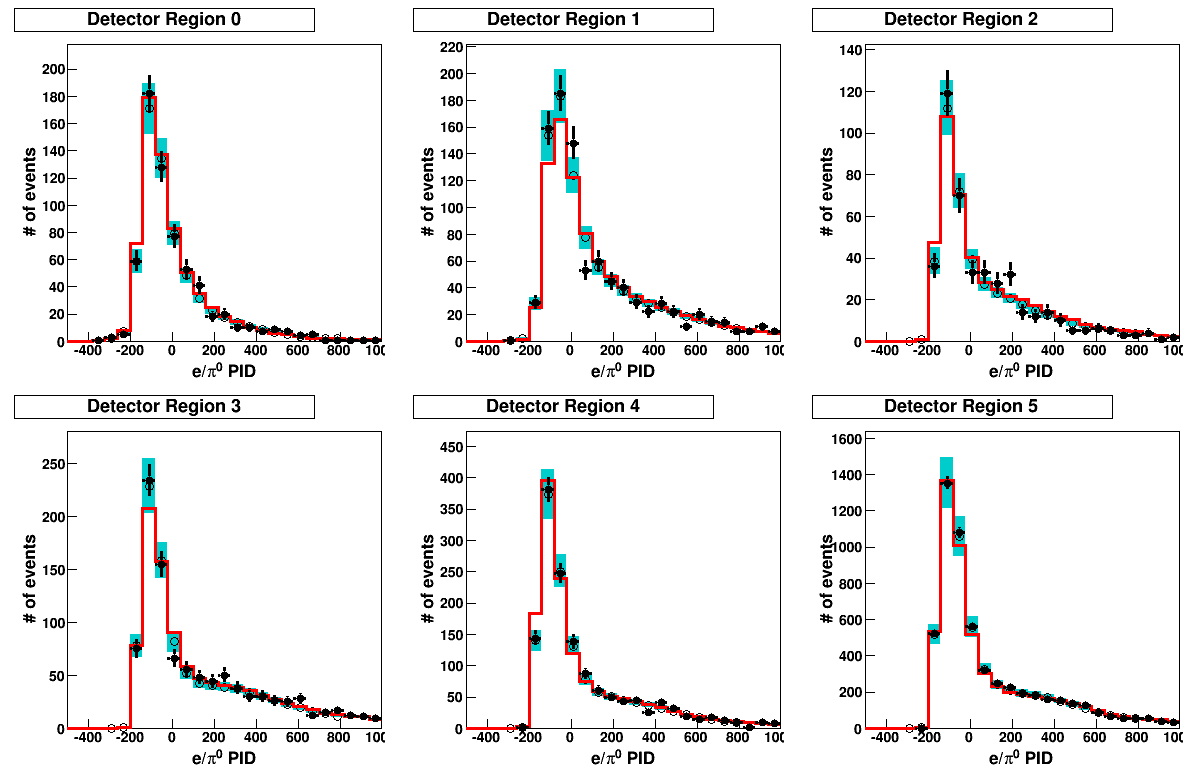
\includegraphics[width=0.9\textwidth]{demcmc_fitresult_samp0_attribute1} 
  \end{center}
  \caption{Fit results for the $l=0$ control sample (no decay electrons) for
  the fiTQun $e/\pi^{0}$ PID variable in each of the detector regions. Positive
  values denote more $\pi^{0}$-like events, negative values denote more
  $e$-like events. Red histogram shows nominal MC prediction.  Black points
  represent observed data.  Teal histogram shows post-fit distribution, where
  the mean is the average of the DE-MCMC throws and the error bar is the square
  root of the variance.}
  \label{fig:fitresults_samp0_att1}
\end{figure}


\begin{figure}[h]
  \begin{center}
    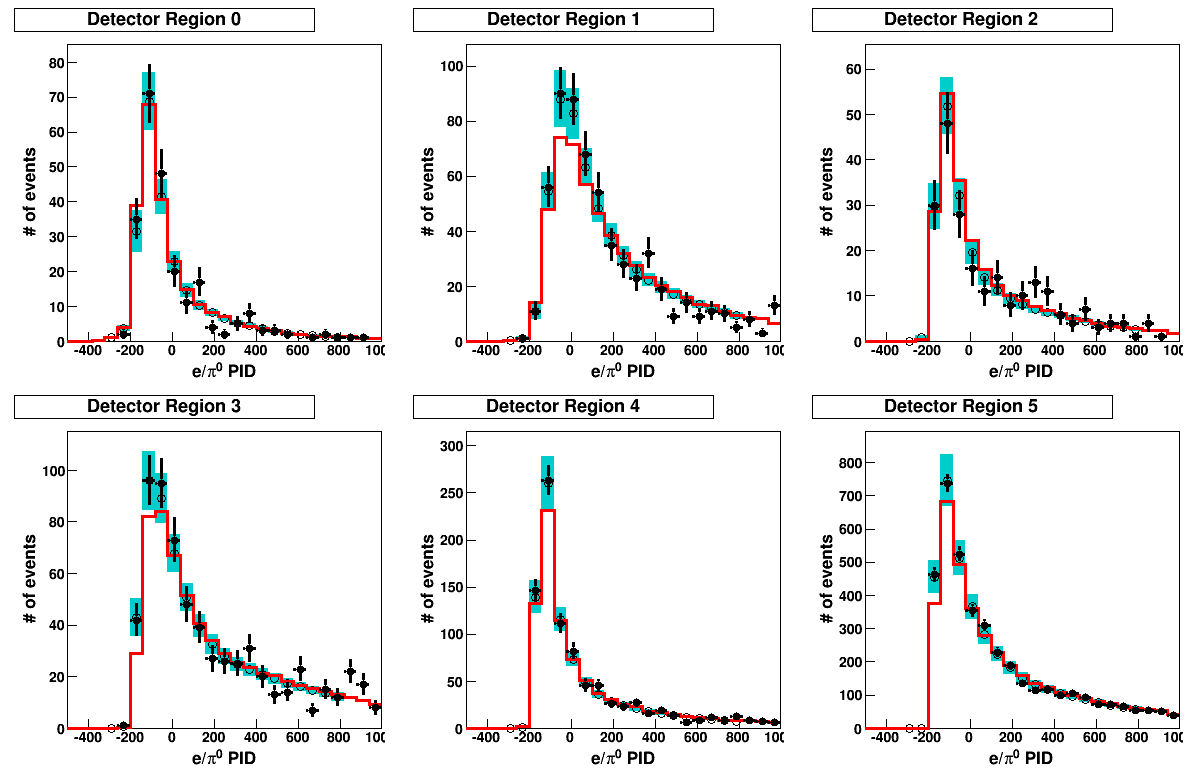
\includegraphics[width=0.9\textwidth]{demcmc_fitresult_samp1_attribute1} 
  \end{center}
  \caption{Fit results for the $l=1$ control sample (one decay electron) for
  the fiTQun $e/\pi^{0}$ PID variable in each of the detector regions. Positive
  values denote more $\pi^{0}$-like events, negative values denote more
  $e$-like events. Red histogram shows nominal MC prediction.  Black points
  represent observed data.  Teal histogram shows post-fit distribution, where
  the mean is the average of the DE-MCMC throws and the error bar is the square
  root of the variance.}
  \label{fig:fitresults_samp1_att1}
\end{figure}


\begin{figure}[h]
  \begin{center}
    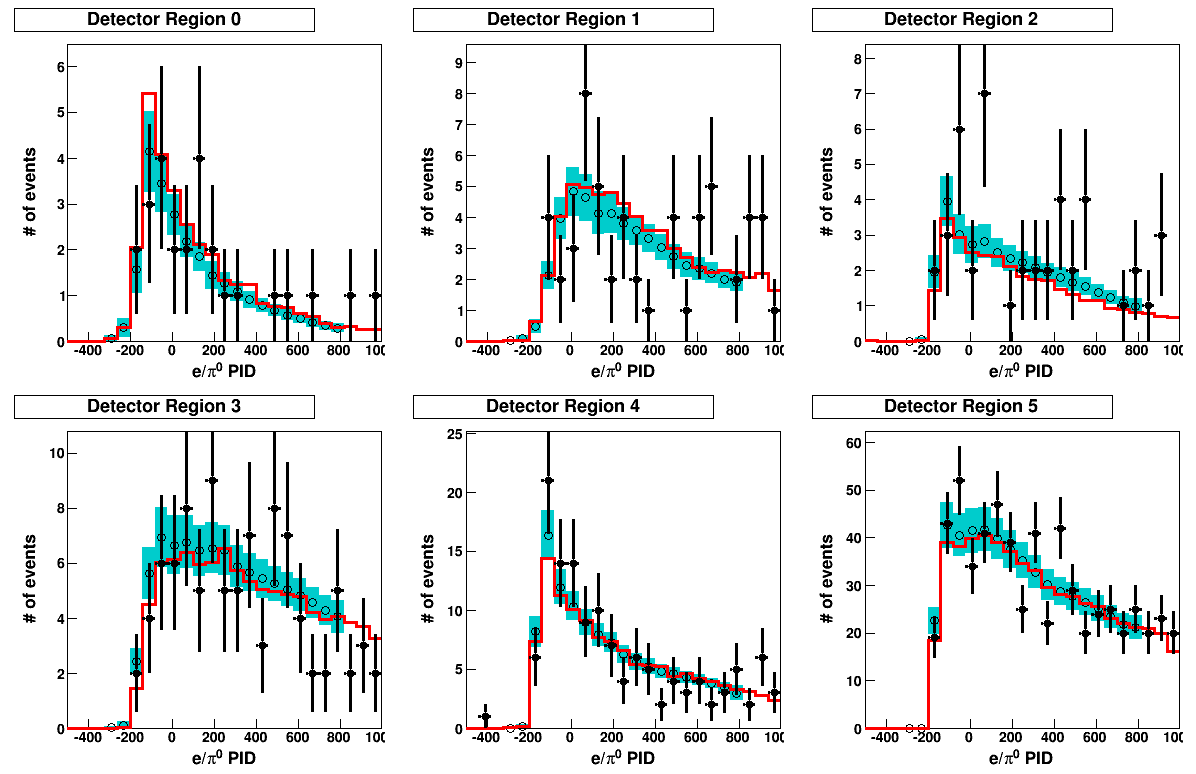
\includegraphics[width=0.9\textwidth]{demcmc_fitresult_samp2_attribute1} 
  \end{center}
  \caption{Fit results for the $l=2$ control sample (more than one decay
  electron) for the fiTQun $e/\pi^{0}$ PID variable in each of the detector
  regions.  Positive values denote more $\pi^{0}$-like events, negative values
  denote more $e$-like events. Red histogram shows nominal MC prediction.
  Black points represent observed data.  Teal histogram shows post-fit
  distribution, where the mean is the average of the DE-MCMC throws and the
  error bar is the square root of the variance.}
  \label{fig:fitresults_samp2_att1}
\end{figure}


%% ATTRIBUTE 2 %%%%%%%%%%%%%%%%%%%%%%%%%%%%%%%%%%%%%%%%%%%%%%%%%%%%%%%%%%%%%%%%%%%
\begin{figure}[h]
  \begin{center}
    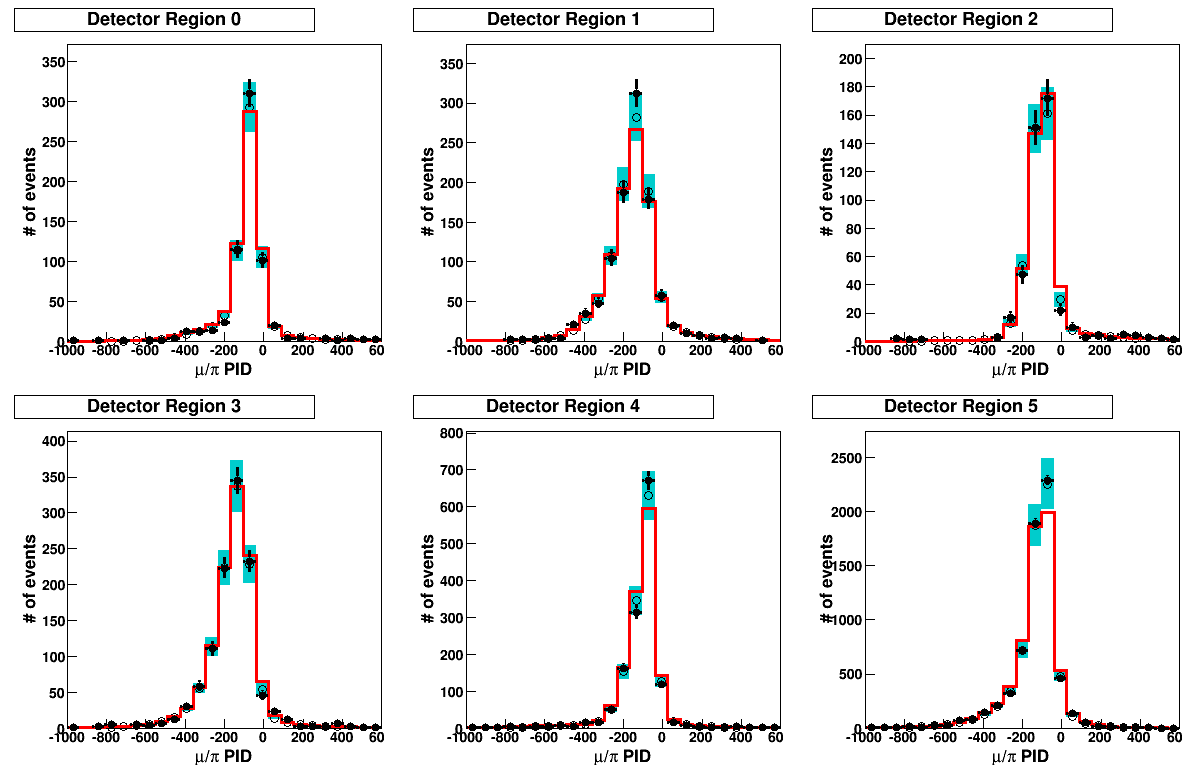
\includegraphics[width=0.9\textwidth]{demcmc_fitresult_samp0_attribute2} 
  \end{center}
  \caption{Fit results for the $l=0$ control sample (no decay electrons) for
  the fiTQun $\mu/\pi$ PID variable in each of the detector regions. Positive
  values denote more $\pi$-like events, negative values denote more $\mu$-like
  events. Red histogram shows nominal MC prediction.  Black points represent
  observed data.  Teal histogram shows post-fit distribution, where the mean is
  the average of the DE-MCMC throws and the error bar is the square root of the
  variance.}
  \label{fig:fitresults_samp0_att2}
\end{figure}


\begin{figure}[h]
  \begin{center}
    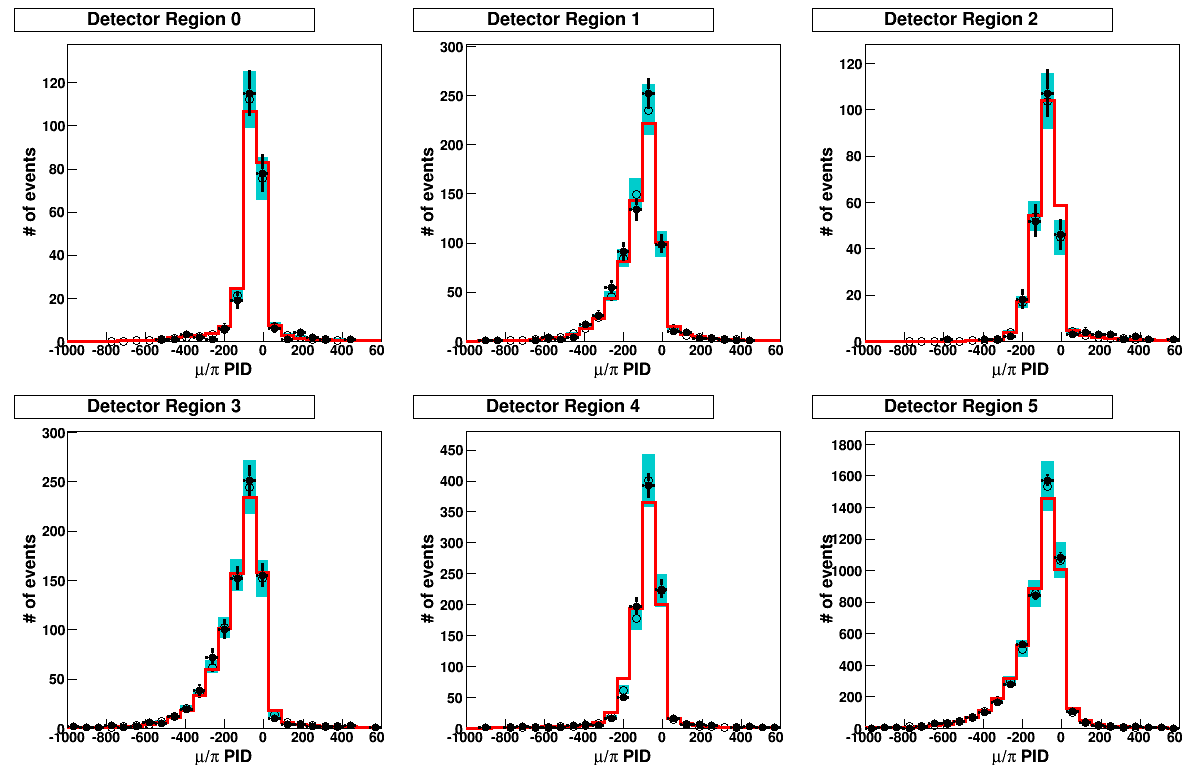
\includegraphics[width=0.9\textwidth]{demcmc_fitresult_samp1_attribute2} 
  \end{center}
  \caption{Fit results for the $l=1$ control sample (one decay electron) for
  the fiTQun $\mu/\pi$ PID variable in each of the detector regions.  Positive
  values denote more $\pi$-like events, negative values denote more $\mu$-like
  events. Red histogram shows nominal MC prediction.  Black points represent
  observed data.  Teal histogram shows post-fit distribution, where the mean is
  the average of the DE-MCMC throws and the error bar is the square root of the
  variance.} 
  \label{fig:fitresults_samp1_att2}
\end{figure}


\begin{figure}[h]
  \begin{center}
    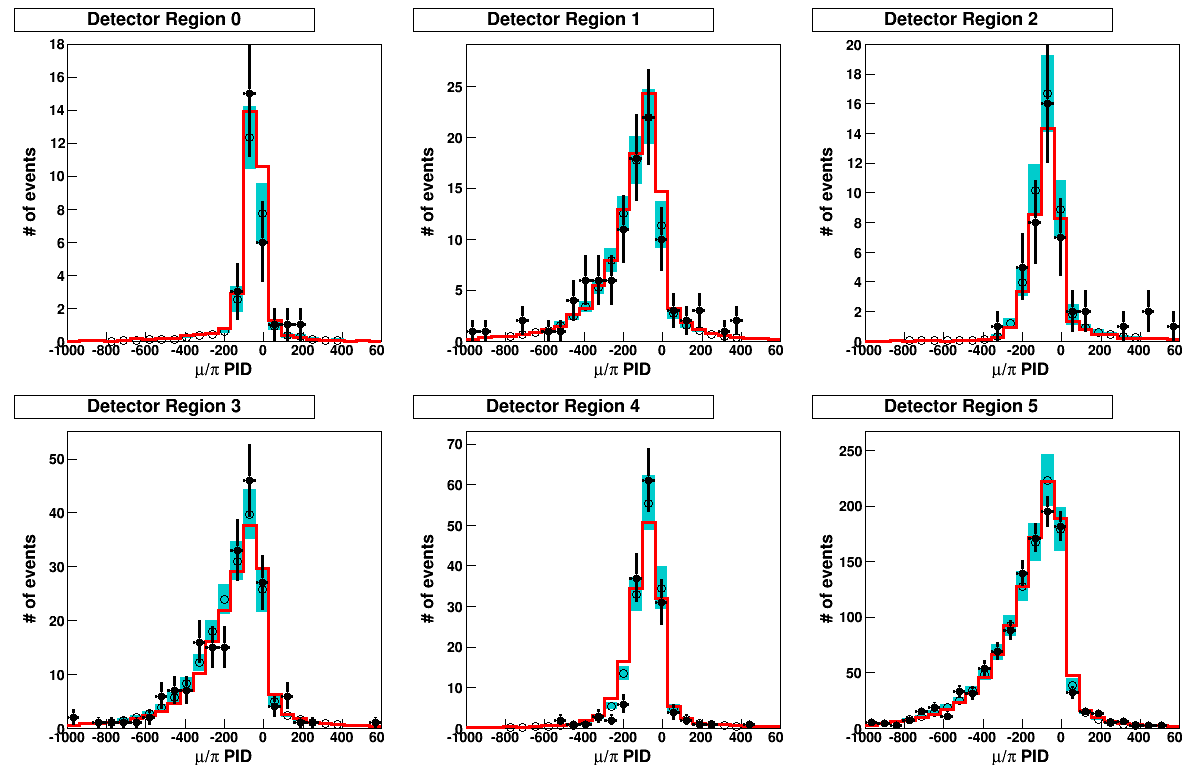
\includegraphics[width=0.9\textwidth]{demcmc_fitresult_samp2_attribute2} 
  \end{center}
  \caption{Fit results for the $l=2$ control sample (more than one decay
  electron) for the fiTQun $\mu/\pi$ PID variable in each of the detector
  regions.  Positive values denote more $\pi$-like events, negative values
  denote more $\mu$-like events. Red histogram shows nominal MC prediction.
  Black points represent observed data.  Teal histogram shows post-fit
  distribution, where the mean is the average of the DE-MCMC throws and the
  error bar is the square root of the variance.}
  \label{fig:fitresults_samp2_att2}
\end{figure}


%% ATTRIBUTE 3 %%%%%%%%%%%%%%%%%%%%%%%%%%%%%%%%%%%%%%%%%%%%%%%%%%%%%%%%%%%%%%%%%%%
\begin{figure}[h]
  \begin{center}
    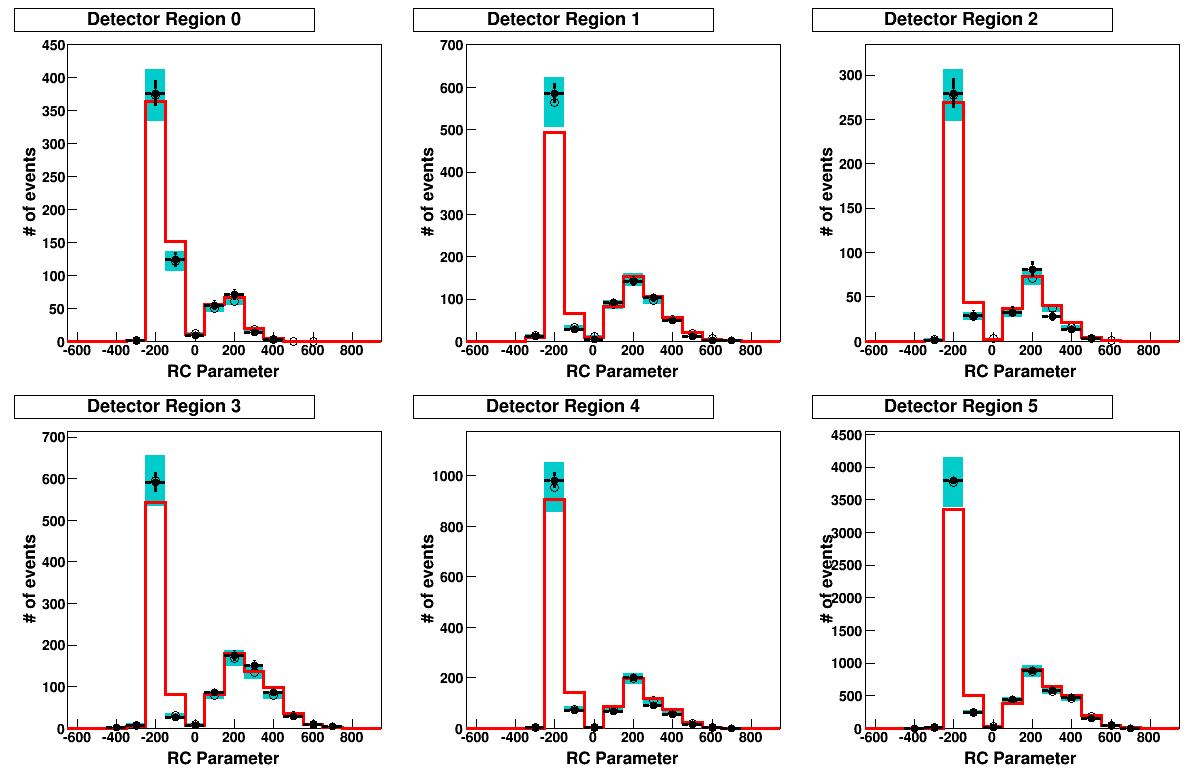
\includegraphics[width=0.9\textwidth]{demcmc_fitresult_samp0_attribute3} 
  \end{center}
  \caption{Fit results for the $l=0$ control sample (no decay electrons) for
  the fiTQun RC (ring-counting) variable in each of the detector regions.
  Positive values denote more multi-ring-like events, negative values denote
  more single-ring-like events. Red histogram shows nominal MC prediction.
  Black points represent observed data.  Teal histogram shows post-fit
  distribution, where the mean is the average of the DE-MCMC throws and the
  error bar is the square root of the variance.}
  \label{fig:fitresults_samp0_att3}
\end{figure}


\begin{figure}[h]
  \begin{center}
    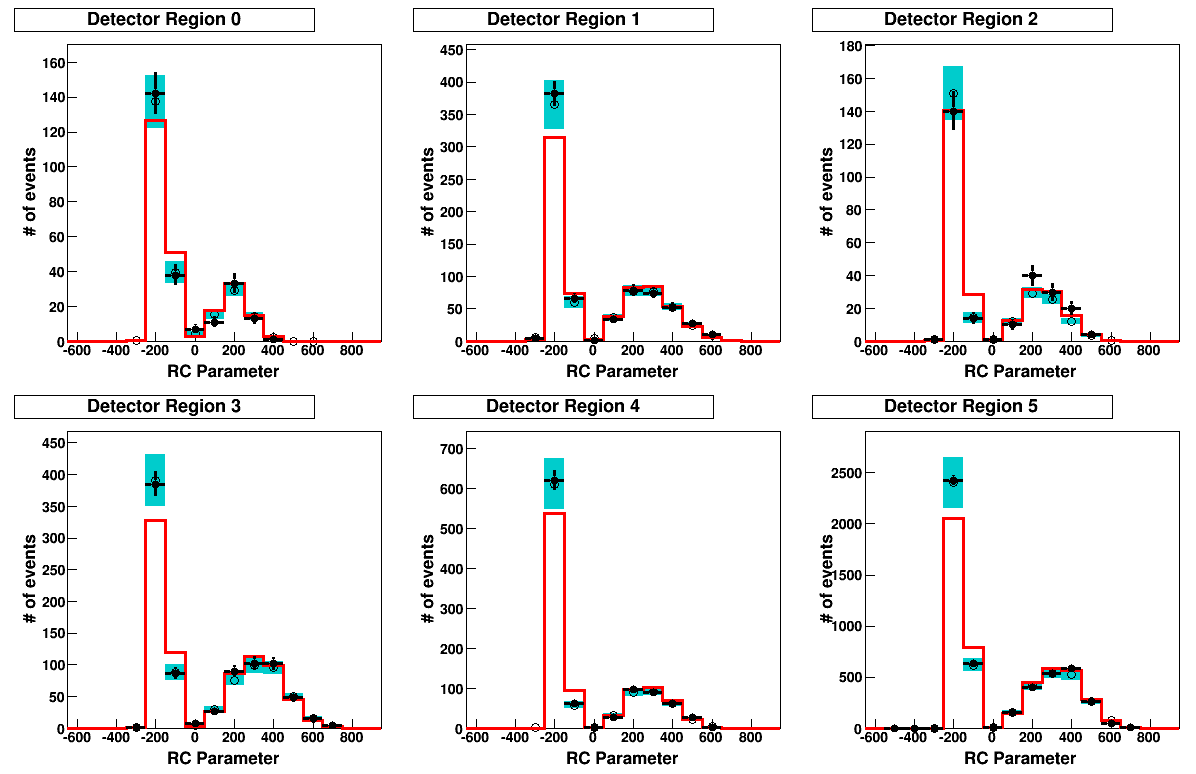
\includegraphics[width=0.9\textwidth]{demcmc_fitresult_samp1_attribute3} 
  \end{center}
  \caption{Fit results for the $l=1$ control sample (one decay electron) for
  the fiTQun $\mu/\pi$ PID variable in each of the detector regions.  Positive
  values denote more multi-ring-like events, negative values denote more
  single-ring-like events. Red histogram shows nominal MC prediction.  Black
  points represent observed data.  Teal histogram shows post-fit distribution,
  where the mean is the average of the DE-MCMC throws and the error bar is the
  square root of the variance.}
  \label{fig:fitresults_samp1_att3}
\end{figure}


\begin{figure}[h]
  \begin{center}
    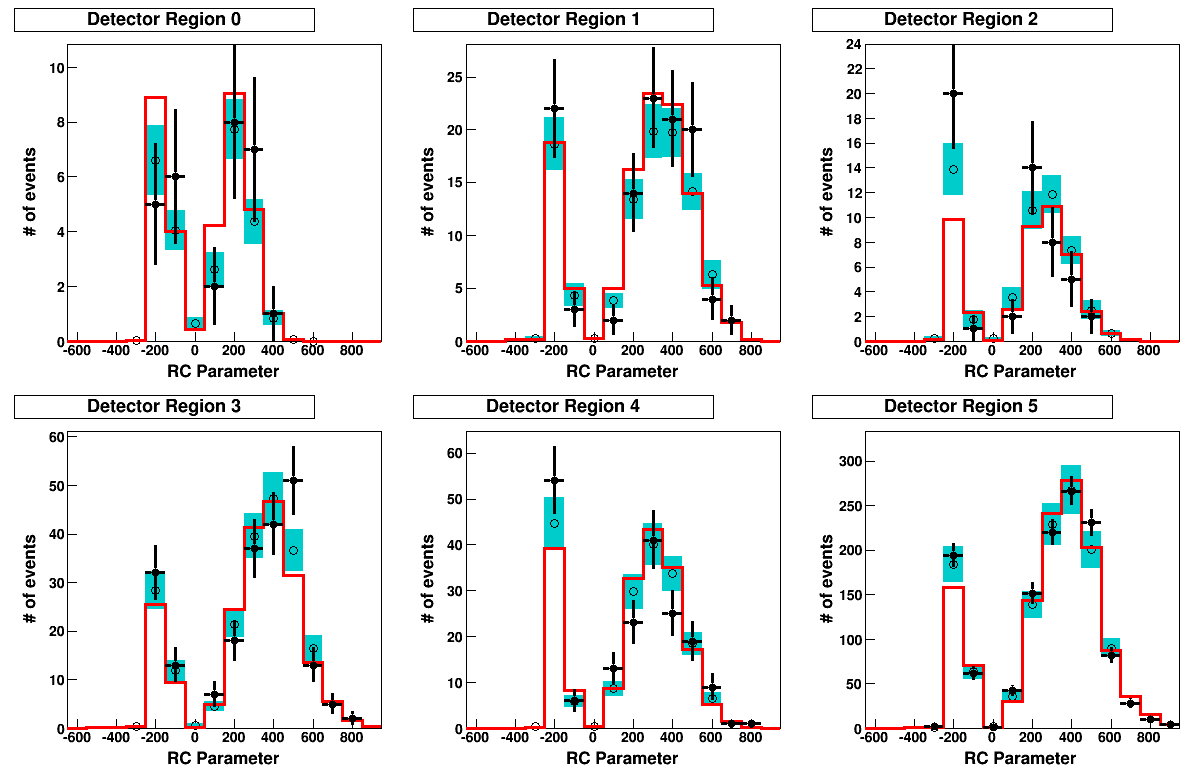
\includegraphics[width=0.9\textwidth]{demcmc_fitresult_samp2_attribute3} 
  \end{center}
  \caption{Fit results for the $l=2$ control sample (more than one decay
  electron) for the fiTQun $\mu/\pi$ PID variable in each of the detector
  regions.  Positive values denote more multi-ring-like events, negative values
  denote more single-ring-like events.  Red histogram shows nominal MC
  prediction.  Black points represent observed data.  Teal histogram shows
  post-fit distribution, where the mean is the average of the DE-MCMC throws
  and the error bar is the square root of the variance.}
  \label{fig:fitresults_samp2_att3}
\end{figure}


%
%\begin{figure}[h]
%  \begin{center}
%   \centering
%   \begin{tabular}[h]{l l}
%    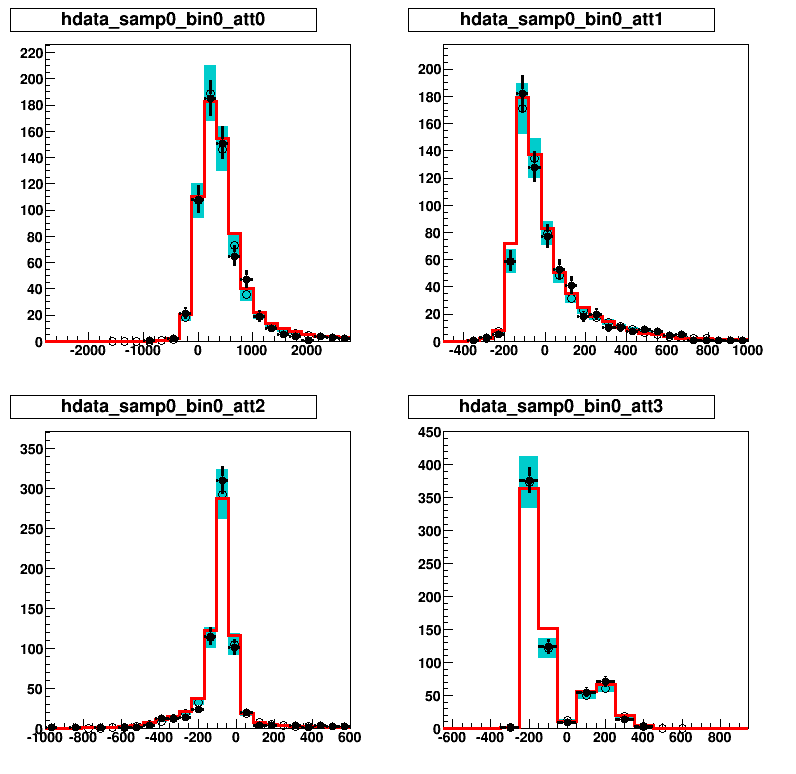
\includegraphics[width=0.55\textwidth]{demcmc_fitresult_samp0_bin0} 
%     &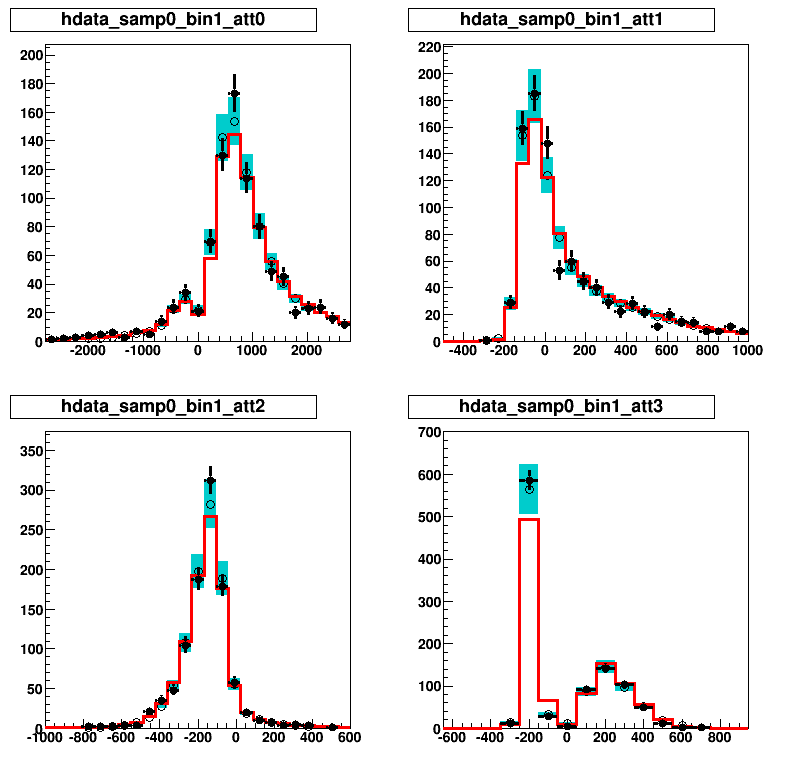
\includegraphics[width=0.55\textwidth]{demcmc_fitresult_samp0_bin1} \\
%     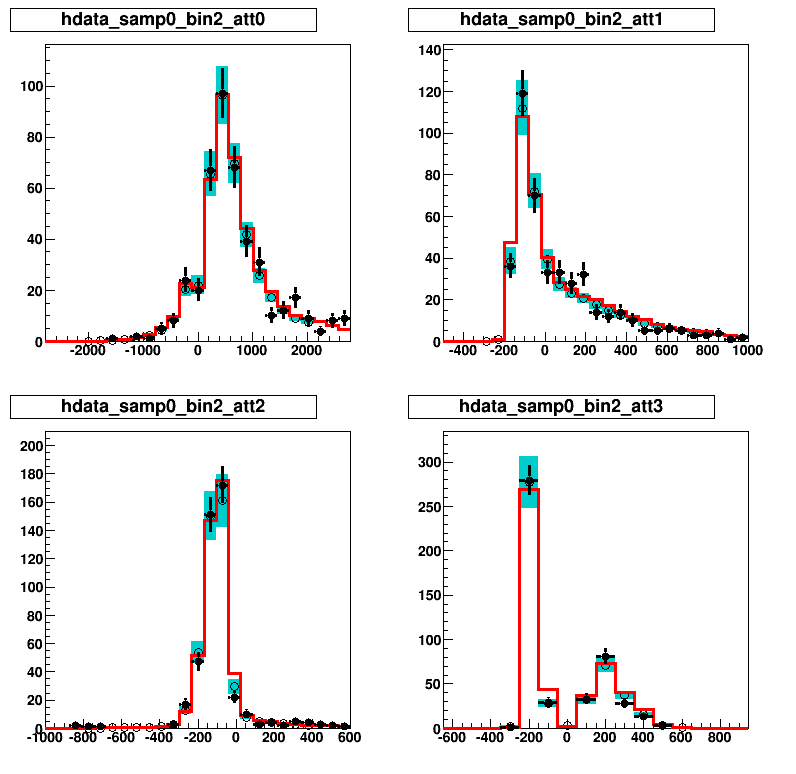
\includegraphics[width=0.55\textwidth]{demcmc_fitresult_samp0_bin2}   
%     &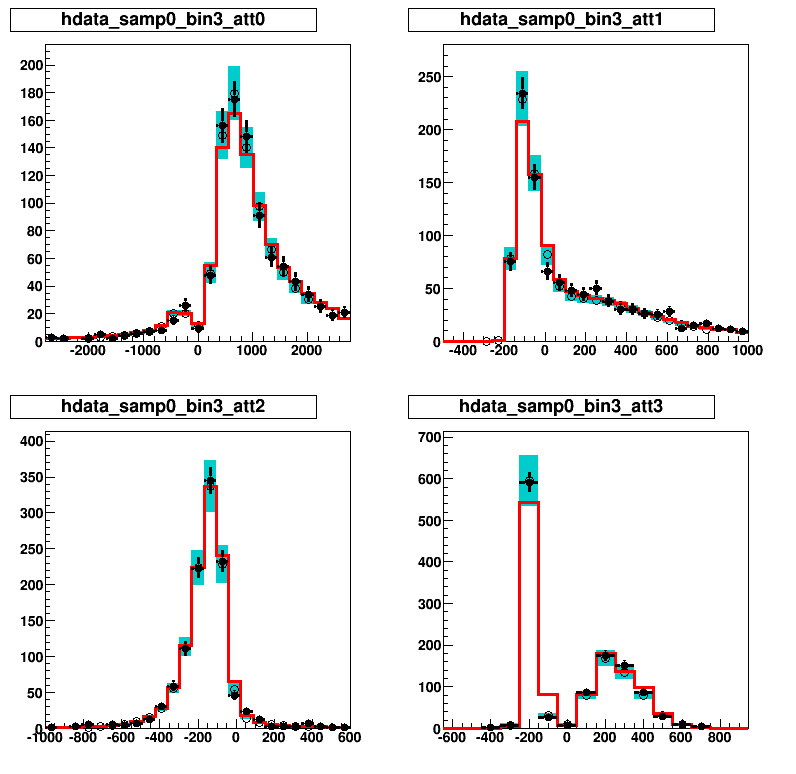
\includegraphics[width=0.55\textwidth]{demcmc_fitresult_samp0_bin3} \\ 
%     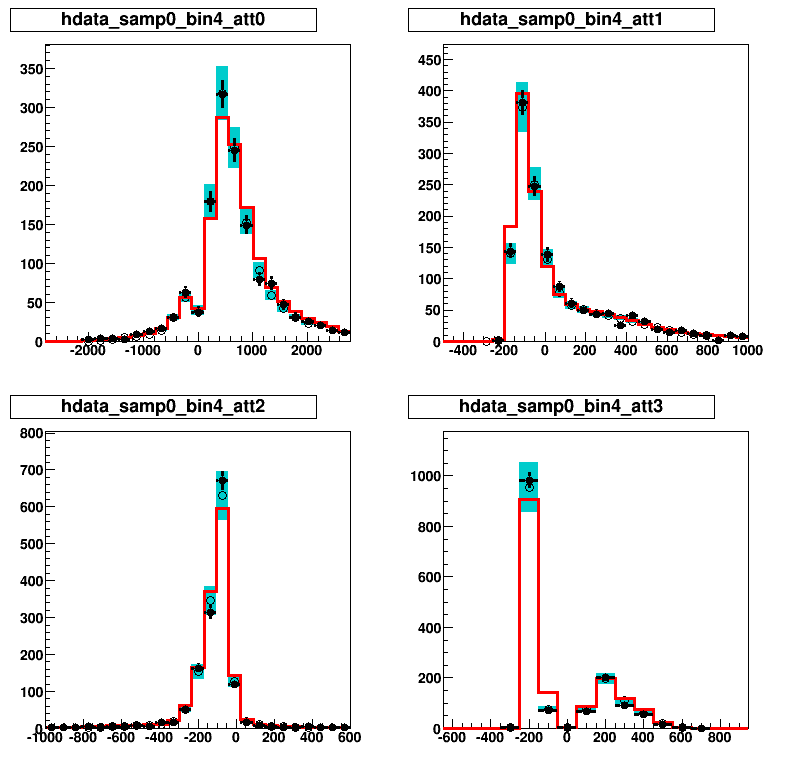
\includegraphics[width=0.55\textwidth]{demcmc_fitresult_samp0_bin4} 
%     &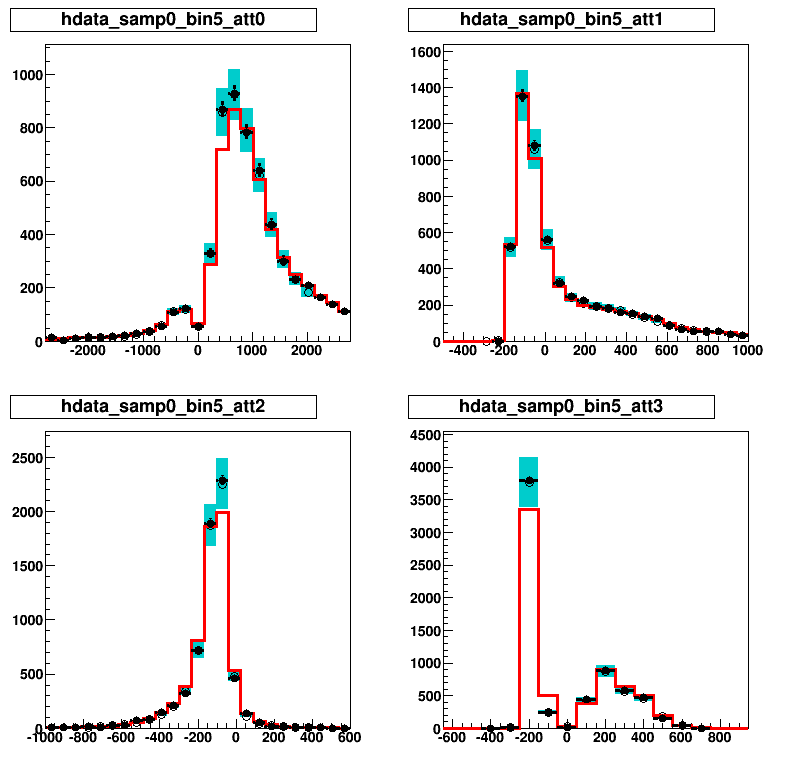
\includegraphics[width=0.55\textwidth]{demcmc_fitresult_samp0_bin5} 
%  \end{tabular}
%  \end{center}
%  \caption{Fit results for the $l=0$ control sample (no decay electrons) for each
%  fiTQun cut variable in each of the detector regions. Red histogram shows
%  nominal MC prediction.  Black points represent observed data.  Teal histogram
%  shows post-fit distribution, where the mean is the average of the DE-MCMC
%  throws and the error bar is the square root of the variance.}
%  \label{fig:fitresults_samp0}
%\end{figure}
%
%
%\begin{figure}[h]
%  \begin{center}
%   \begin{tabular}[h]{c c c}
%     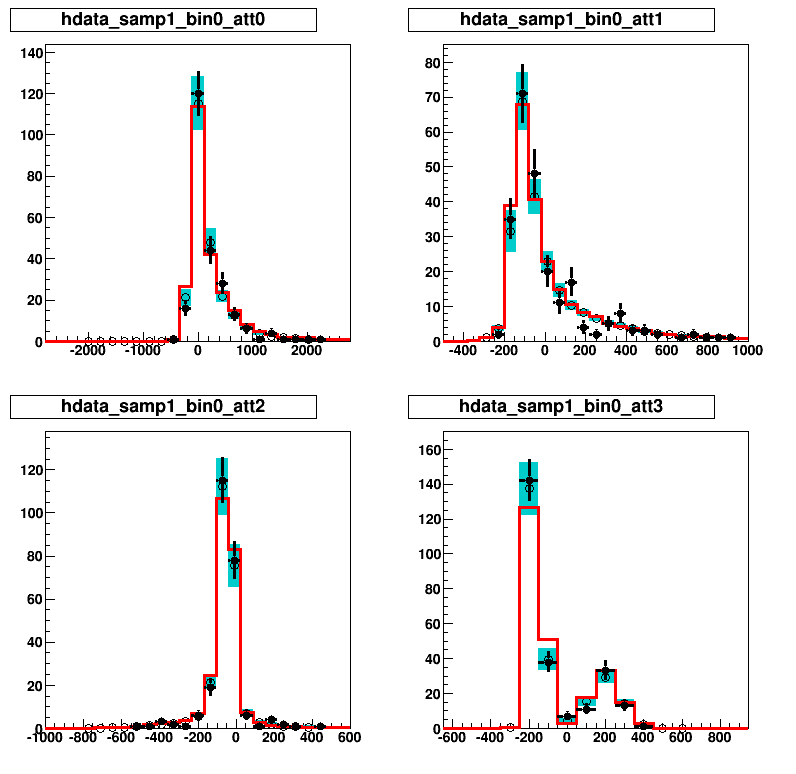
\includegraphics[width=0.33\textwidth]{demcmc_fitresult_samp1_bin0} 
%      &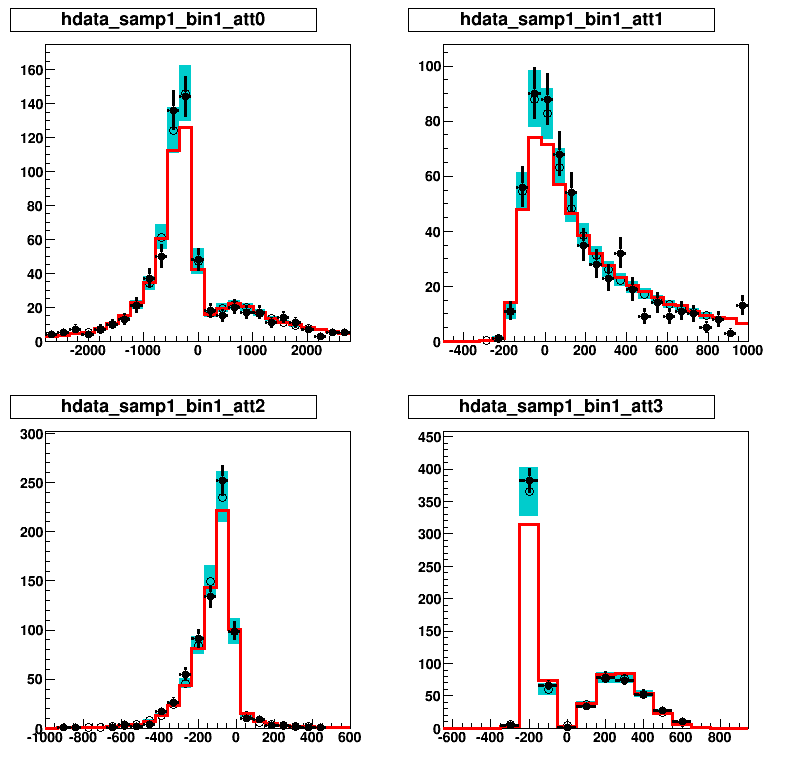
\includegraphics[width=0.33\textwidth]{demcmc_fitresult_samp1_bin1} 
%      &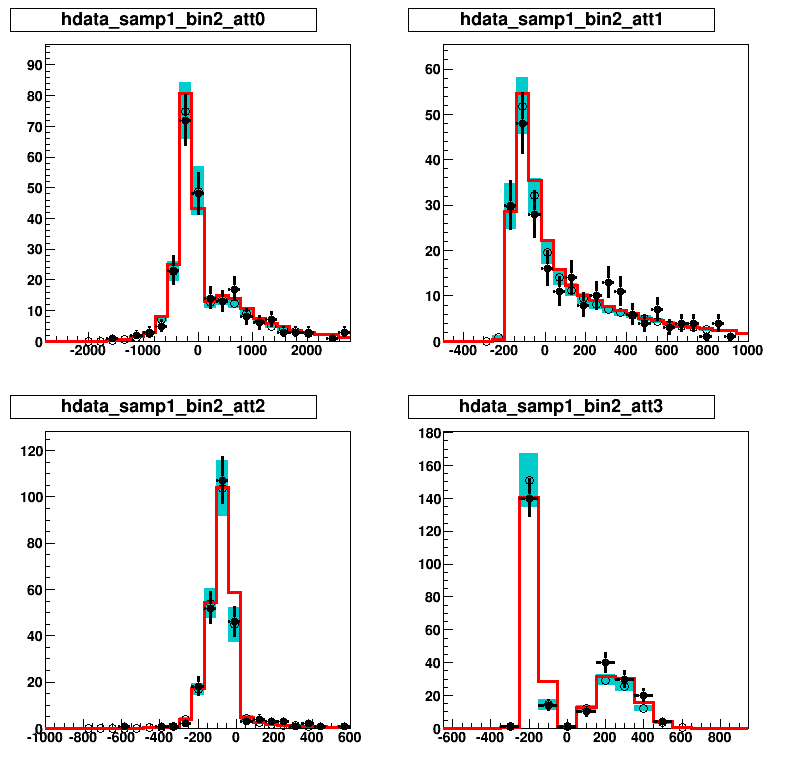
\includegraphics[width=0.33\textwidth]{demcmc_fitresult_samp1_bin2}  \\ 
%      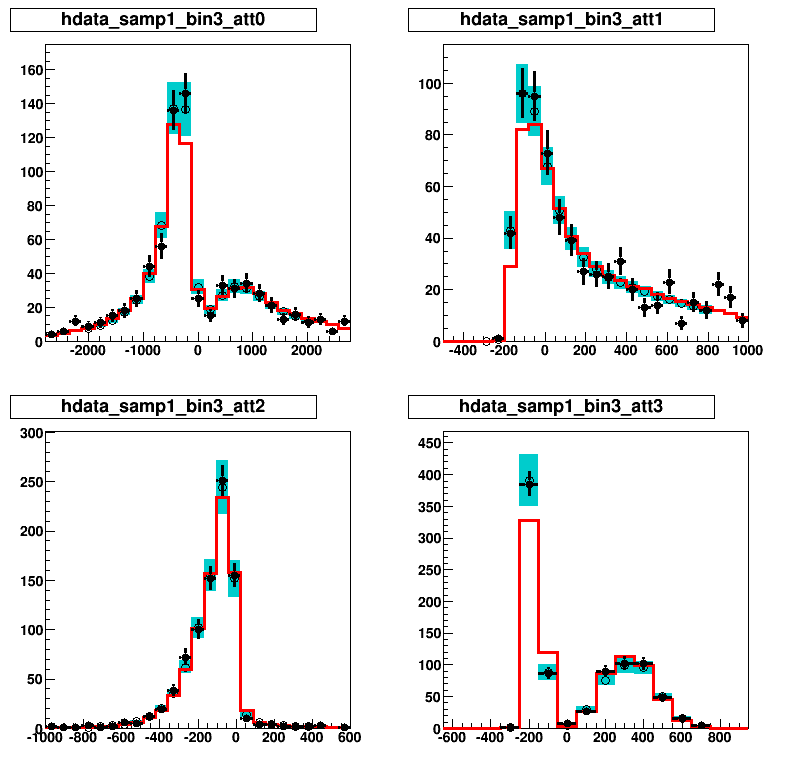
\includegraphics[width=0.33\textwidth]{demcmc_fitresult_samp1_bin3} 
%      &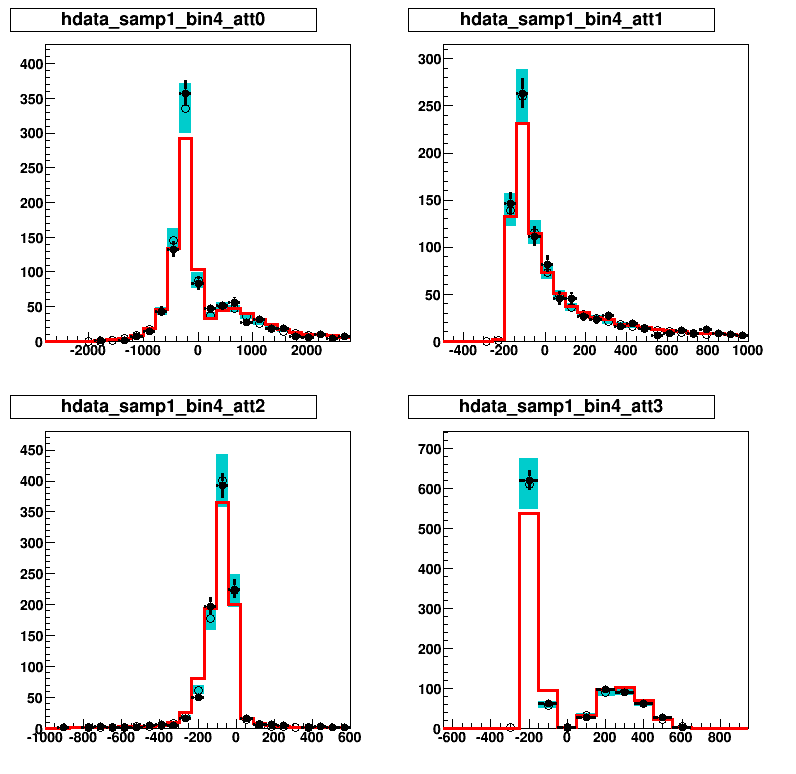
\includegraphics[width=0.33\textwidth]{demcmc_fitresult_samp1_bin4} 
%      &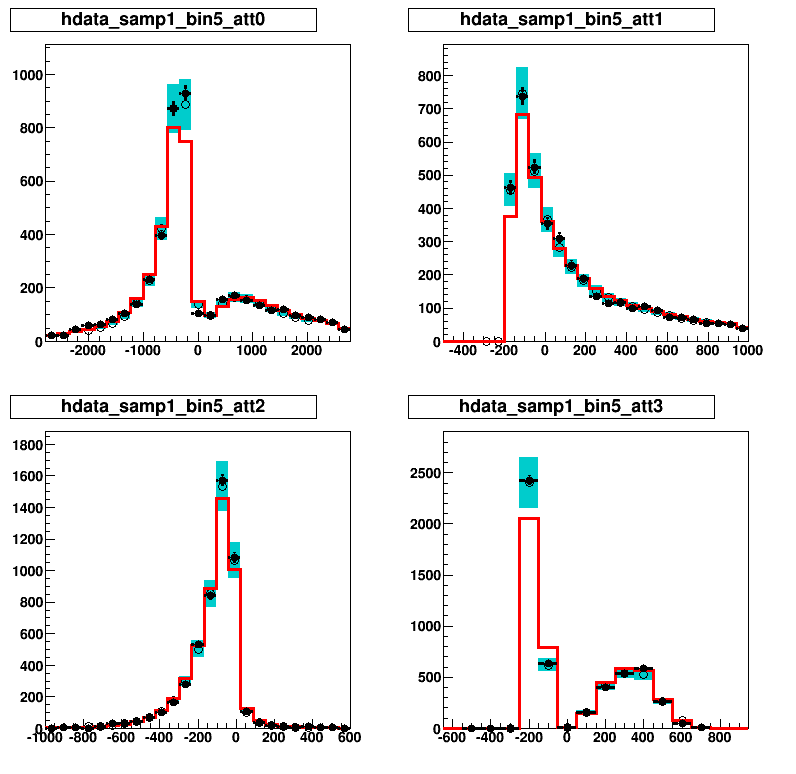
\includegraphics[width=0.33\textwidth]{demcmc_fitresult_samp1_bin5} 
%  \end{tabular}
%  \end{center}
%  \caption{Fit results for the $l = 1$ control sample (one decay electron) for each
%  fiTQun cut variable in each of the detector regions. Red histogram shows
%  nominal MC prediction.  Black points represent observed data.  Teal histogram
%  shows post-fit distribution, where the mean is the average of the DE-MCMC
%  throws and the error bar is the square root of the variance.}
%  \label{fig:fitresults_samp1}
%\end{figure}
%
%
%\begin{figure}[h]
%  \begin{center}
%   \begin{tabular}[h]{c c c}
%     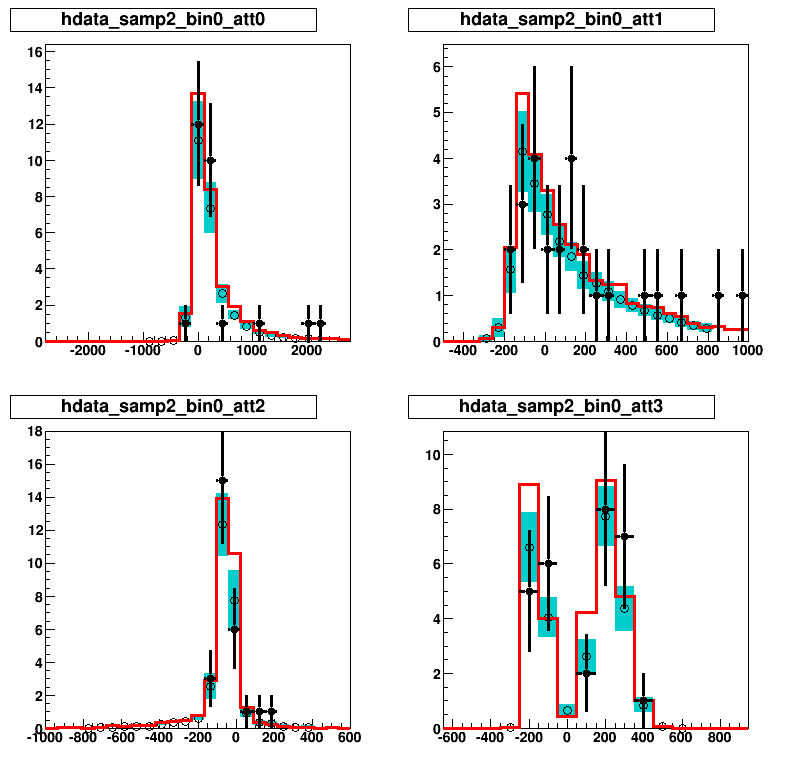
\includegraphics[width=0.33\textwidth]{demcmc_fitresult_samp2_bin0} 
%      &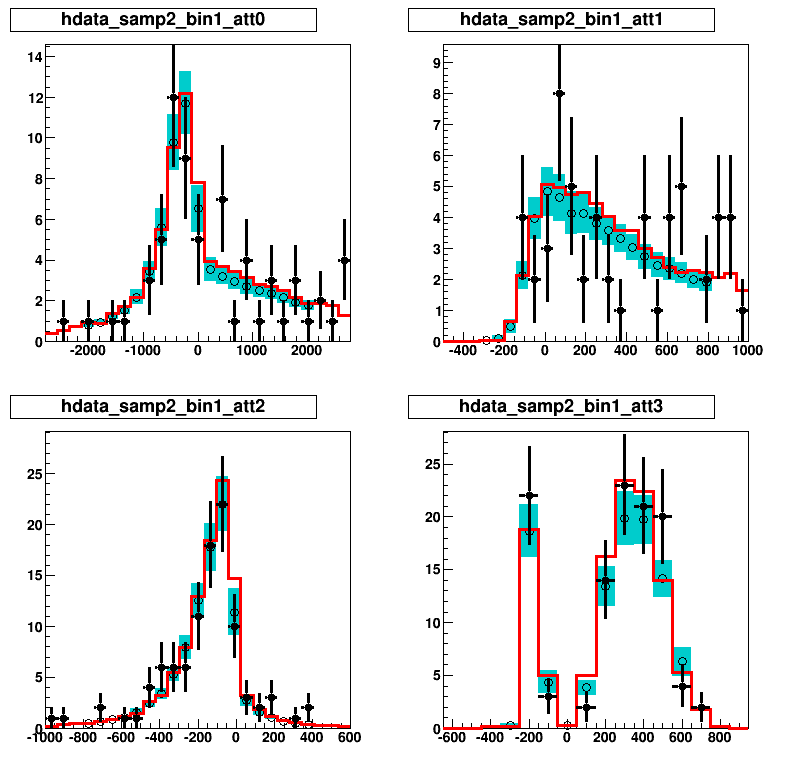
\includegraphics[width=0.33\textwidth]{demcmc_fitresult_samp2_bin1} 
%      &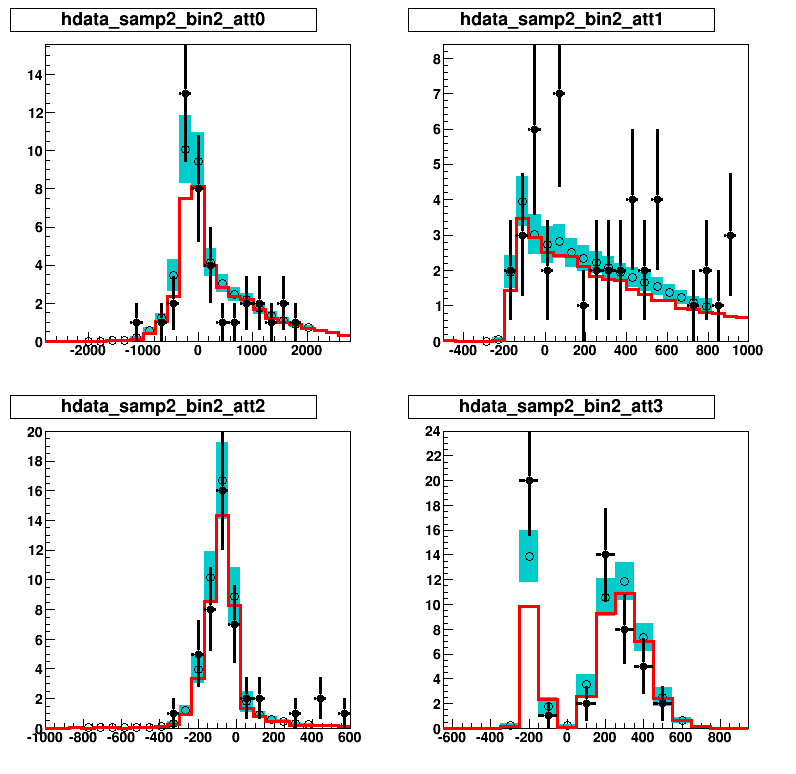
\includegraphics[width=0.33\textwidth]{demcmc_fitresult_samp2_bin2}  \\ 
%      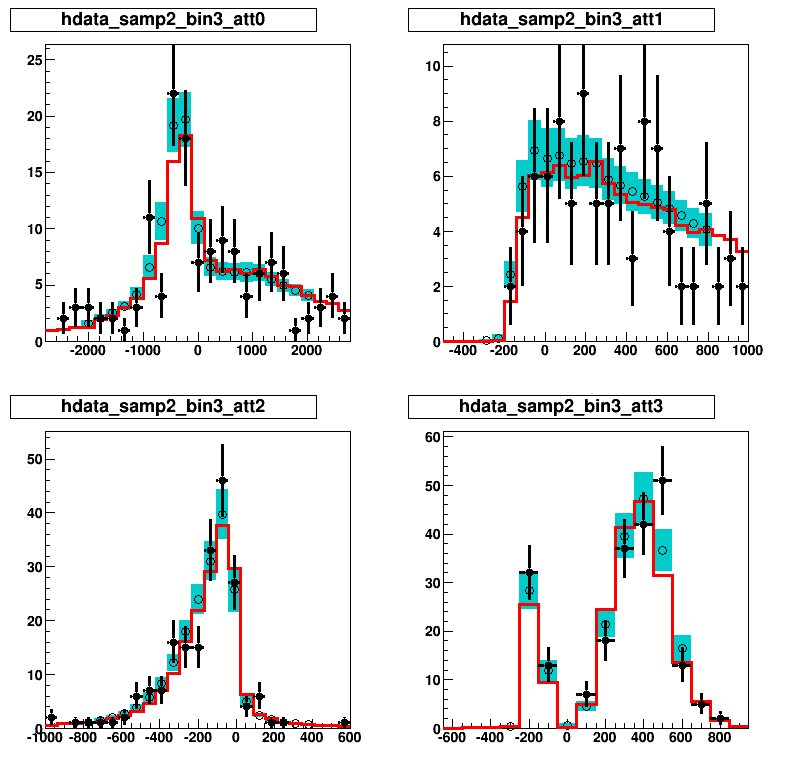
\includegraphics[width=0.33\textwidth]{demcmc_fitresult_samp2_bin3} 
%      &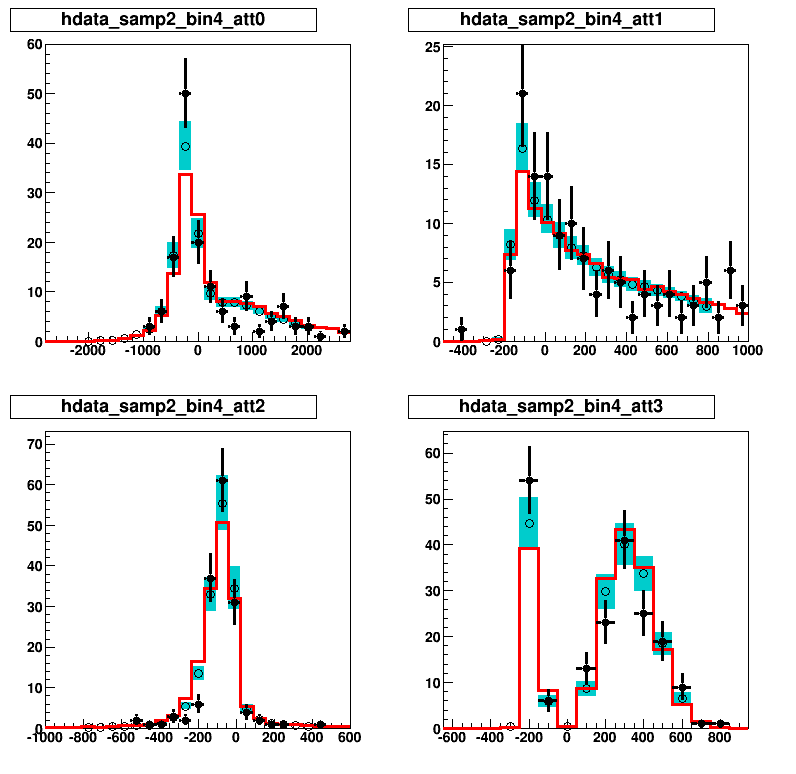
\includegraphics[width=0.33\textwidth]{demcmc_fitresult_samp2_bin4} 
%      &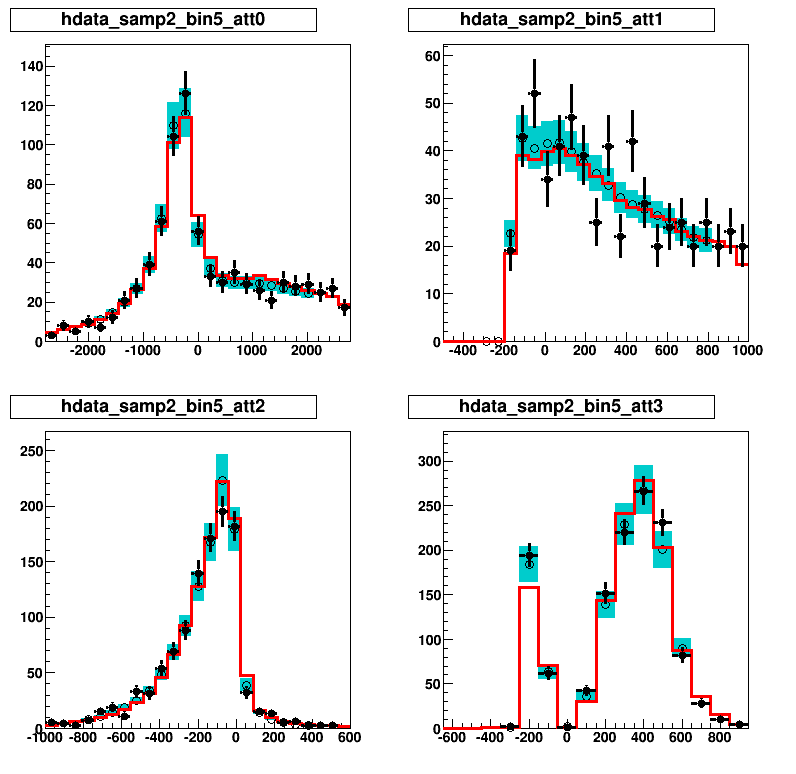
\includegraphics[width=0.33\textwidth]{demcmc_fitresult_samp2_bin5} 
%  \end{tabular}
%  \end{center}
%  \caption{Fit results for the $l = 2$ control sample (more than one decay electron) for each
%  fiTQun cut variable in each of the detector regions. Red histogram shows
%  nominal MC prediction.  Black points represent observed data.  Teal histogram
%  shows post-fit distribution, where the mean is the average of the DE-MCMC
%  throws and the error bar is the square root of the variance.}
%  \label{fig:fitresults_samp2}
%\end{figure}

%-----------------------------------------------------------------------------
